\documentclass[12pt,twoside]{article}
\usepackage{light}
\usepackage{subfigure}
\usepackage{graphicx}
%\hidesolutions
\showsolutions


\begin{document}
\newcommand{\proofrubric}[3][Any correct proof.]
  {
  	\begin{center}
	\fbox{\begin{minipage}{35em}
	\textbf{Rubric}
	\par
	[#3pts] #1
		\begin{center}
		\textbf{or}
		\end{center}
	#2
	\end{minipage}}
	\end{center}
  }
  
  \newcommand{\rubric}[1]
  {
  	\begin{center}
	\fbox{\begin{minipage}{35em}
	\textbf{Rubric}
	\par
	#1
	\end{minipage}}
	\end{center}
  }

\problemset{5}{October 4, 2016}{Wednesday, October 12} 
\noindent \textbf{Reading Assignment:}   Sections 5.2, 6.3
\\




\begin{problem}{20}  The following series of problems deals with the notion of Hamiltonian cycles and Eulerian circuits in undirected graphs.  A Hamiltonian cycle is a path that visits each vertex of a graph exactly once and ends at its starting vertex.  An Eulerian circuit is a path that traverses all edges of a graph exactly once and ends at its starting vertex.  A useful fact for this series of problems is that a connected graph has an Eulerian circuit if and only if all vertices of the graph have even degree (you may use this fact without proof throughout the problems).

\bparts

\ppart{5} Is it true that if a simple graph has an Eulerian circuit, then it has a Hamiltonian cycle? If yes, then provide a proof.  Otherwise, provide a counterexample.
\rubric{
[2pts] No. \par
[3pts] Correct counterexample.
}
\solution{
This is not true.  Consider a graph that is two triangles joined together at one vertex.  The graph has an Eulerian circuit as we can visit the edges of the first triangle and then visit the edges of the second triangle and return back to the connecting vertex.  However, the graph has no Hamiltonian cycles since this would involve visiting the connecting vertex twice.  
}

\ppart{5} Is it true that if a simple graph has an Hamiltonian cycle, then it has a Eulerian circuit? If yes, then provide a proof.  Otherwise, provide a counterexample.
\rubric{
[2pts] No. \par
[3pts] Correct counterexample.
}
\solution{
This is also not true.  Consider the complete graph on four vertices $K_4$.  Each vertex of this graph has odd degree so there cannot be an Eulerian circuit, but there is a Hamiltonian cycle: just traverse the four nodes in order using the outer edges.  
}

\ppart{10}

            \begin{figure}[!ht]
                \begin{center}
                    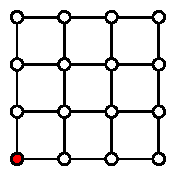
\includegraphics[scale=1.5]{ps5-figs/GridGraph.pdf}
                \caption{4 x 4 grid graph}
                \label{1-fig1}
            \end{center}
            \end{figure}

Bruce missed out on trick-or-treating as a kid.  However, at the ripe age of 22, Bruce decides to dress up as Batman and try out trick-or-treating for the first time.  Suppose that the above graph represents Bruce's neighborhood with each edge representing some street that is lined with houses and Bruce's home being the lower left corner vertex (colored red).  Bruce wants to visit all the streets to get as much candy as possible, but doesn't get any candy from re-visiting a street.  What is the fewest number of streets Bruce has to revisit in order to visit all the streets in his neighborhood and return home?  
\eparts
\rubric{
[10pts] 4 streets \par
\begin{center}
\textbf{or}
\end{center}
[5pts] Wrong number of streets but some reasoning.
}
\solution{
The fewest number of streets Bruce has to revisit in order to visit all the streets in his neighborhood and return home is 4.  Translating the problem into graph theory, we are looking for the minimum number of edges that need to be traversed twice in an Eulerian circuit starting at Bruce's house.  

We first note that Bruce's neighborhood has exactly 8 vertices of odd degree (degree 3).  We know that if a graph has all vertices of even degree, then the graph has an Eulerian circuit.  So we try to make this graph into a graph with all vertices of even degree by adding in as few edges as possible such that traversing an added edge means traversing an edge in the original graph again.  

We construct the following new graph shown in Figure 2 below:
            \begin{figure}[!th]
                \begin{center}
                    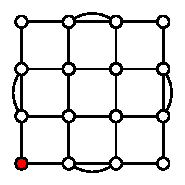
\includegraphics[scale=1.5]{ps5-figs/GridGraphSolution.pdf}
                \caption{4 x 4 grid graph}
                \label{1-fig1}
            \end{center}
            \end{figure}

Now each vertex in the graph has even degree and so it has an Eulerian circuit.  Now traversing any of the added edges in our Eulerian circuit means that the actual edge in the graph was traversed twice.  Hence the number of edges that need to be revisited in Bruce's neighborhood is four.  Now this is the minimum number of edges that need to be revisited because each traversal of edges back to the starting vertex with revisited edges corresponds to a new graph with additional edges drawn between adjacent vertices.  However, connecting any other pair of adjacent vertices creates at least one odd degree vertex, which will then require us to add in more correcting edges in order to create a graph with an Eulerian circuit.  

}

\end{problem}



% P1
\begin{problem}{15} 

  In the cycle $C_{2n}$ of length $2n$, we'll call two vertices
  \emph{opposite} if they are on opposite sides of the cycle, that is
  that are distance $n$ apart in $C_n$.  Let $G$ be the graph formed
  from $C_{2n}$ by adding an edge, which we'll call a \emph{crossing
    edge}, between each pair of opposite vertices.  So $G$ has $n$
  crossing edges.

\bparts

\ppart{5} Give a simple description of the shortest path between any two
vertices of $G$.

\emph{Hint: Argue that a shortest path between two vertices in $G$ uses at
most one crossing edge.}
\rubric{
[1pts] Shortest path has two possibilities (choose the shorter one). \par
[2pts] Uses crossing edge and then follows path to the end vertex. \par
[2pts] Follows path from one vertex to the other without a crossing path.
}
\solution{
  Suppose a path, $Q$, in $G$ begins with a crossing edge, then
  follows a path, $P$, in $C_{2n}$ and ends with another crossing
  edge.  Replacing every vertex in $P$ by its opposite, you get a walk
  in $C_{2n}$ between the endpoints of $Q$, but the new walk is two
  edges shorter than $Q$.  This implies that a \emph{shortest} path in
  $G$ uses at most one crossing edge.

  A path $Q$ that uses exactly one crossing edge will have the
  following form: it follows a path $P_1$ in $C_{2n}$, then a crossing edge,
  and then another path $P_2$ in $C_{2n}$. We could describe another
  path by first following a crossing edge, then all of the
  opposite edges of path $P_1$, and then $P_2$; this path has the same
  length.

  So it suffices to consider the following two candidates for the shortest
  path from $v$ and $w$.
  The first candidate follows a crossing edge to the opposite $v'$ of $v$,
  and then navigates around the cycle $C_{2n}$ to the target vertex $w$. The
  second candidate uses no crossing edges, and simply navigates around
  $C_{2n}$. The first of these has length $1 + c_{v'w}$, and the second
  of these has length $c_{vw}$; so to find a shortest path from $v$ to
  $w$, we compare these two quantities and choose either the first or
  second candidate to yield the smaller length.

  We can even write $c_{v'w} = n - c_{vw}$; then we choose the first candidate
  when $1 + n - c_{vw} \leq c_{vw}$, i.e.\ when $c_{vw} \geq \frac{n+1}{2}$,
  and otherwise choose the second candidate.
}

\ppart{3} What is the \emph{diameter} of $G$, that is, the largest
distance between two vertices?
\rubric{
[3pts]  $n=2k$ the diameter is $k$, and if $n=2k+1$, the diameter is $k + 1$, $\left \lceil{n/2}\right \rceil$
\begin{center}
\textbf{or}
\end{center}
[2pts] $\frac{n}{2}$ without consideration of even or odd $n$.
}
\solution{
    If $n=2k$ the diameter is $k$.  If $n = 2k + 1$ the diameter
  is also $k$.  (For $d \in [1,n)$ find the maximum value of
    $\min(d,1+n-d)$.)
}

\ppart{3} We say that a graph is \emph{$k$-edge connected} if removing
  $(k-1)$ edges can not disconnect the graph. Prove that the graph above is
  not 4-edge connected.
\rubric{
[3pts] Remove all edges connected to a vertex.
}
\solution{
    Every vertex of the graph has degree $3$.  Removing all $3$
  edges incident to a vertex disconnects the graph.  (If it was
  $4$ connected, no matter what $3$ edges we remove, the graph would
  have to remain connected.)
  }

\ppart{4} Prove that the graph is 3-edge connected.
\proofrubric{
[2pts] Removing two edges in $C_{2n}$ splits it into two connected components.\par
[2pts] Adding an edge from one connected component to the other connected component that was opposite connects the two connected components.
}{4}
\solution{
    Let $G'$ be the graph that remains after removing two edges.
  Removing any two edges that were orginally part of $C_{2n}$ splits
  $C_{2n}$ into two connected components, each of them paths.  Call
  them $P$ and $P'$.  Since the length of the paths and the two
  removed edges sum to $2n$, one path must have length at most $n-1$.
  Call this one $P$.  Pick a vertex $v$ within $P$.  $v$ is distance
  $n$ to some other vertex, $w$, in $C_{2n}$.  So $w$ must be in the
  other path $P'$.  The paths $P$, $P'$, and the edge $(v,w)$
  form a spanning tree in $G'$ which then must be connected.

  Removing at most one edge from $C_{2n}$ leaves $C_{2n}$ connected,
  hence $G'$ remains connected too.
  }

\eparts
\end{problem}




\begin{problem}{10} Consider a Hunger Games scenario in which a tribute must be selected from a set of boys and a second tribute must be selected from a set of girls.  However, suppose that the Hunger Games committee wants to first match each boy with a girl and then simply select a pair from the possible matchings.  Suppose that the committee lets each boy rank each of the girls he wants to be paired with and vice-versa.  Prove or disprove the following claim: for
some $n \geq 3$ ($n$ boys and $n$ girls, for a total of $2n$ people), there exists a set of boys' and girls' rankings such that any matching made by the committee is stable.\\
\proofrubric{
[2pts] False. \par
[3pts] For every set, there is a girl that is rated worst by at least $n - 2$ boys. Or, there will be at least 2 boys who do not rate a girl at the bottom of their list. Partial credit of 1 point may be given if they say 1. \par
[5pts] Some sort of simulation where that girl is paired a boy that is at the bottom and the two cases where:
\begin{itemize}
	\item $[$2pts] the boy has her at the bottom of his list or
	\item $[$2pts] the boy does not have her at the bottom of his list and show that
	\item $[$1pt] both cases result in a rogue couple because there is at least one other boy who does not have her at the bottom of his list.
\end{itemize}
[-2pts] Any incorrect logic.

}{10}
\solution{
The claim is false.

\begin{proof} We will use letters to denote girls and numbers to denoted boys.

There must be some girl $A$ rated worst by at most $n-2$ boys.  The
reason is as follows.  Each boy can rate exactly one girl worst.  If
each of the $n$ girls was rated worst by at least $n-1$ boys, then
there would have to be at least $n (n-1)$ boys in all.  But this is
false when $n \geq 3$, because then $n (n-1)$ exceeds $n$, the actual
number of boys.

Suppose that this girl $A$ is paired with the boy, 1, that she rates
worst.  Since at most $n-2$ boys rate girl $A$ worst, there is some
other boy, 2, that rates a different girl, $B$, worst.  Suppose that
boy 2 is paired with girl $B$.

Now girl $A$ and boy $2$ form a rogue couple.  Girl $A$ prefers every
other boy to her current matching, 1.  Similarly, boy $2$ prefers every other girl
to his current matching $B$.  Therefore, $A$ and boy $2$ prefer one another to their
current matchings.
\end{proof}
}
\end{problem}















% P5
\begin{problem}{10}
    
    Show that the congestion of the $N$-input butterfly is $\sqrt{N}$ if $N$ is an even power of $2$.
\proofrubric{
[3pts] Some observation about how congestion relates to level the node is at. Number of outputs have to be matched to the number of inputs and is $\min \{ 2^i, 2^{n-i} \}$ at a level $i$. \par
[3pts] Congestion is $2^{\frac{n}{2}}$ at the middle level.\par
[3pts] Conclusion that congestion of $\sqrt{N}$ is achieved in middle level because $\sqrt{N} = 2^{\frac{n}{2}}$. \par
[1pt] Something to show that the congestion of an $N$ input butterfly is exactly $\sqrt{N}$ when $n$ is even.
}{10}
    \solution{
        First we will show that the congestion is at most $\sqrt{N}$.

        Let $v$ be an arbitrary vertex at some level $i$. Let $S_v$ be the set of inputs that can reach vertex $v$. Let $T_v$ be the set of outputs that are reachable from vertex $v$. Note that:
        \begin{itemize}
            \item For the butterfly network, there is a unique path from each input to each output, so the congestion is the maximum number of messages passing through a vertex for any matching of inputs to outputs.
            \item If $v$ is a vertex at level $i$ of the butterfly network, there is a path from exactly $2^i$ input vertices to $v$ and a path from $v$ to exactly $2^{n-i}$ output vertices.
        \end{itemize}

        We thus have $|S_v| = 2^i$ and $|T_v| = 2^{n-i}$. The number of inputs in $S_v$ that are matched with outputs in $T_v$ is at most $\min \{ 2^i, 2^{n-i} \}.$ To obtain an upper-bound on the congestion of the network, we need to find the maximum value of $\min \{ 2^i, 2^{n-i} \}$, where the maximum is taken over all $i$. The maximum value is achieved when $2^i$ and $2^{n-i}$ are as equal as possible. Since $n$ is even, these two quantities are equal when $i = \frac{n}{2}$, hence the maximum congestion is $2^{n/2} = N^{1/n} = \sqrt{N}$.

        So far, we have concluded that the congestion of $\sqrt{N}$ can only be achieved at a node at level $\frac{n}{2}$. Now consider the node at that level whose binary representation is all $0$s. Any packet from the input in the form $z\underbrace{0\ldots000}_{n/2\text{ bits}}$ with destination $\underbrace{000\ldots0}_{n/2\text{ bits}} z'$, where $z$ and $z'$ are any $\frac{n}{2}$-bit numbers, must pass through this node. In the worst case, all packets from input in the form $z\underbrace{0\ldots000}_{n/2\text{ bits}}$ will have destination in the form $\underbrace{000\ldots0}_{n/2\text{ bits}} z'$. But there are $2^{n/2} = \sqrt{N}$ such possible packets, giving the node load $\sqrt{N}$. Therefore, we can conclude that the congestion of $B_n$ is exactly $\sqrt{N}$ when $n$ is even.
    }

\end{problem}









% P6
\begin{problem}{20}

    In a \emph{perfect shuffle}, a deck of $N$ cards is cut exactly in half and then perfectly interlaced. Thus, for $N$ cards, we would obtain the resulting cards in the following order:
    $$ 1,\; \left(\frac{N}{2} + 1\right),\; 2,\; \left(\frac{N}{2} + 2\right),\; \ldots,\; \left(\frac{N}{2} - 1\right),\; \left(N - 1\right),\; \frac{N}{2},\; N. $$

    \bparts

    \ppart{10} Show that $m$ perfect shuffles will return a deck of $N$ cards to its original order provided that $2^m = 1 \pmod{(N-1)}$.
\rubric{
[10pts] Any correct reasoning.
\begin{center}
\textbf{if they did not use switches}
\end{center}
[-1pt] Math errors. \par
[2pts] Top card and bottom card do not change position. \par
[2pts] Card in top half end up at $2i$. (Note numbers might be different if they do not 0-index).\par
[2pts] Cards in bottom half end up at $2(i-\frac{N}{2}) + 1$. \par
[2pts] Some writing of indices using remainders or mod. \par
[2pts] $m$ shuffles results in $2^m i \equiv i \pmod{(N-1)}$ where card at index $i$ returns to index $i$
}
    \solution{
        Let $N \times m$ switches $P_0^1,\; P_1^1,\; \ldots,\; P_{N-1}^m$ be available, where $N = 2^m$ for some positive integer $m$. In this network of $N \times m$ switches, there is a one-way link connecting $P_i$ to $P_j$, where $j = 2i$ for $0 \leq i \leq \frac{N}{2} - 1$ and $j = 2i + 1 - N$ for $\frac{N}{2} \leq i \leq N - 1$.

        Now, let the binary representation of $i$ be $b_{m-1} b_{m-2} \ldots b_1 b_0$, where $b_k$ is $0$ or $1$, for $0 \leq k \leq m-1$. Then, the binary representation of $j$ is $b_{m-2} b_{m-3} \ldots b_0 b_{m-1}$, so that:
        \begin{align*}
            i &= b_{m-1} 2^{m-1} + b_{m-2} 2^{m-2} + \ldots + b_1 2 + b_0, \\
            j &= b_{m-2} 2^{m-1} + b_{m-3} 2^{m-2} + \ldots + b_0 2 + b_{m-1}. \\
        \end{align*}
        We see that the binary representation of $j$ is obtained by cyclically shifting the binary representation of $i$ one position to the right. For example, when $m=3$, we have:
        $$ 000 \to 000,\; 001 \to 100,\; 010 \to 001,\; 011 \to 101, $$
        $$ 100 \to 010,\; 101 \to 110,\; 110 \to 011,\; 111 \to 111. $$

        We see in Figure 4, where ecah of the eight cards is represented by a $3$-digit binary sequence, this deck of cards is returned to its original order after $3$ perfect shuffles.

        Since $2^m \equiv 1 \pmod{(N-1)}$, we could map $m$ applications of the perfect-shuffle onto a network of $m$ columns of $N$ switches, interconnected by the one-way link described earlier. Given that each binary digit of the input data returns to its original position at the output, $m$ perfect shuffles will return a deck of $N$ cards to its original order.

        \emph{Another approach to this problem:} Let us first identify a pattern in how $N$ cards shift during a perfect shuffle. We have two sets of cards that are produced from the cut, namely the top portion $T$ and the bottom portion $B$. Note that the first card of $B$ is is the original $0$th-position card (here we count the stack of cards from bottom up), and the first card of $T$ was formerly in position $\frac{N}{2}$. For the sake of simplicity of this formulation, let us assume that the first card after the first perfect shuffle comes from set $B$ (i.e.\ the $0$th card).

        The cards in set $B$ were originally indexed $0$ through $(\frac{N}{2} - 1)$. After the perfect shuffle, card $i$ in set $B$ will end up in position $2i$ (all the even positions). The cards in set $T$ were originally indexed $\frac{N}{2}$ through $(N-1)$, and each card $i$ of this set will end up in position $2(i - \frac{N}{2}) + 1$ (all the odd positions). For easy mapping, we now index both $B$ and $T$ starting with $0$: for set $B$, $(0,1,2,3,\ldots) \to (0,2,4,6,\ldots)$, and for set $T$, $(0,1,2,3,\ldots) \to (1,3,5,7,\ldots)$. Now we need to be able to re-index $\frac{N}{2}$ through $(N-1)$ ddown to $0$ through $(\frac{N}{2} - 1)$, which could be achieved by subtracting off $\frac{N}{2}$. Hence we replace $i$ with $(i - \frac{N}{2})$ to get $2(i - \frac{N}{2}) + 1$.

        We can rewrite $2(i - \frac{N}{2})+1$ as $2i - N + 1$, and then as $2i - (N-1)$. Essentially, all cards, regardless of being in $B$ or $T$, will be mapped as $i \mapsto \mathrm{rem}(2i,N-1)$; this term $N-1$ comes from the fact that the top card, in position $(N-1)$, never moves during the shuffle. Note that the $0$th position card never moves either, as reflected by the mapping $2 \cdot 0 = 0$.

        Bringing the above mappings and derivations together, the position of card $i$ after $m$ shuffles will be $\mathrm{rem}(2^m i, N-1)$. We can rewrite this as $2^m i \equiv r \pmod{(N-1)}$, where $r$ is the resulting position of the card. But we know that $2^m \equiv 1 \pmod{(N-1)}$, so we can multiply both sides by $i$ to obtain $2^m i \equiv i \pmod{(N-1)}$, which means that $r = i$. We conclude that, since $2^m i \equiv i \pmod{(N-1)}$, after $m$ shuffles, card $i$ will return to its original position.
         
    }

    \ppart{5} Show that $8$ perfect shuffles are necessary and sufficient to return a deck of $52$ cards to their original order.
\rubric{
[-1pt] Math errors.\par
[5pts] Substitute 8 in for $m$ and 52 in for $N$.
}
    \solution{
        Substituting $8$ for $m$ and $52$ for $N$, where $m$ and $N$ are related as in part (a), we find from the congruence below that $8$ perfect shuffles are sufficient to return a deck of $52$ cards to their original order:
        \begin{align*}
            2^m &\equiv 1 \pmod{(N-1)} \\
            2^8 &\equiv 1 \pmod{(52 - 1)} \\
            256 &\equiv 1 \pmod{51} \\
            \frac{256-1}{51} &= 5
        \end{align*}

        We also note that $2^m \not\equiv 1 \pmod{(N-1)}$ for $N=52$ and $1 \leq m < 8$. Therefore, $8$ perfect shuffles are necessary to return a deck of $52$ cards to their original order.
    }

    \ppart{5} How many perfect shuffles are necessary and sufficient to return a deck of cards to its original order if there are two jokers added to the deck (so that it has $54$ cards)?
    \rubric{
    [-1pt] Math errors.\par
    [5pts] 52 shuffles.
    }
    \solution{
        The answer is $52$. Note that the top and bottom cards never move. Consider a card $C$ with $i \in \{1,2,\ldots,52\}$ cards above. After $52$ perfect shuffles:
        \begin{align*}
            \text{\# of cards above }C &\equiv 2^{52} \cdot i \pmod{53} \\
                                       &\equiv 1 \cdot i \pmod{53} \\
                                       &\equiv i \pmod {53}.
        \end{align*}
        The second congruence uses Fermat's Theorem, which implies that $2^{52} \equiv 1 \pmod{53}$. If the number of cards above $C$ is congruent to $i \in \{1,2,\ldots,52\}$, then it must be equal to $i$. Thus, every card returns to its original position and the deck is restored after $52$ perfect shuffles.
    }

    \eparts

\end{problem}









% P8
\begin{problem}{10}
    Construct a $16$-bit de Bruijn sequence, by considering an Eulerian tour of the de Bruijn graph.
\rubric{
[10pts] Any Euler tour of a de Bruijin graph. (Make sure every window of three is unique)
}
    \solution{
        We find an Euler tour of the de Bruijn graph, and read off the labels as we traverse the tour: $0111100101000011$.
    }

\end{problem}

\end{document}
